\documentclass{article}
\usepackage{graphicx}
\begin{document}
\title{Labwork 3: Hello CUDA}
\date{October 2024}

\section{Implement the Labwork}
\subsection{Grayscale by CPU}
The input image is read from file, represented as a ndarray in shape of (imageHeight, imageWidth, 3).
I've implemented a loop through all rows and columns of this image, each pixel I did average on (r, g, b) channels.
\begin{verbatim}
def grayscale_cpu(image_file):
  img = plt.imread(image_file)
  out = np.zeros(img.shape, np.uint8)
  start_t = time.time()
  print(f"Do grayscale image by cpu ...")

  for row_idx, row in enumerate(img):
    for col_idx, cell in enumerate(row):
      out[row_idx][col_idx] = [int(np.mean(cell))]*3

  total_time = time.time() - start_t
  print(f"It took {total_time} s to finish.")
  return out, total_time
\end{verbatim}

\subsection{Grayscale by GPU}
\begin{verbatim}
@cuda.jit
def grayscale(src, dst):
  tidx = cuda.threadIdx.x + cuda.blockIdx.x * cuda.blockDim.x
  g = np.uint8((src[tidx, 0] + src[tidx, 1] + src[tidx, 2]) / 3)
  dst[tidx, 0] = dst[tidx, 1] = dst[tidx, 2] = g

def grayscale_gpu(image_file, blockSize=64):
  img = plt.imread(image_file)
  imageHeight, imageWidth, _ = img.shape
  pixelCount = imageWidth * imageHeight
  gridSize = int(pixelCount / blockSize)
  flatSrc = np.reshape(img, (pixelCount, 3))

  print(f"Do grayscale image by gpu, blockSize={blockSize} ...")
  start_t = time.time()

  devSrc = cuda.to_device(flatSrc)
  devDst = cuda.device_array((pixelCount, 3), np.uint8)
  grayscale[gridSize, blockSize](devSrc, devDst)
  hostDst = devDst.copy_to_host()

  total_time = time.time() - start_t
  print(f"It took {total_time} seconds to finish.")

  img = hostDst.reshape((imageHeight, imageWidth, 3))
  return img, total_time
\end{verbatim}

\section{Experiment with different block size values}
I've experimented with block size values of [32, 64, 128, 192, 256, 384, 512, 768, 1024]. The results show that the processing times are not significantly different. (Figure 1)
\begin{figure}
    \centering
    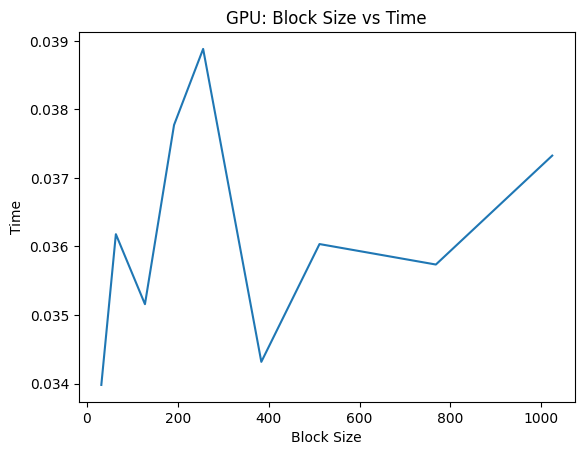
\includegraphics[width=0.5\linewidth]{images/block_time__vs__time.png}
    \caption{Block sizes vs time}
    \label{fig:enter-label}
\end{figure}

\end{document}